\section{Filtering Shared Social Data}
\label{sec:surrounding:360}

The social data of the surrounding scene can be described in different levels of detail. A different ways of describing a surrounding scene include: a 2D image, a panoramic image, a video, a 360-degrees video, a 3D depth image, or a VR 3D model. These different ways of describing the same scene represent the levels of details that can be varied based on the Social AR Continuum and the social proximity between the social contacts. 

This section describes a method and a prototype implementation for filtering shared social data (e.g., 360-degree videos) using wearable AR devices (e.g., HoloLens) \cite{Nassani2018a}. The data filtering is based on the sharer-viewer relationships in order to preserve privacy. For example, when sharing a 360-degrees video, if the user has an intimate relationship with the viewer, then the full fidelity (i.e., the whole 360-degree video) of the sharer's environment is visible. However, if the two are strangers, then only a snapshot image is shared, and the viewer cannot get more information about the sharer's environment. By varying the fidelity of the shared content, the viewer can focus more on the data shared by their close (in terms of social proximity) relations and differentiate this from other content. Also, this approach enables the sharer to have more control over the fidelity of the content shared with their contacts for privacy.

% In this work, we are trying to answer the question, what would be the best way to share rich data (such as 360 videos) within a large social network? The hypothesis is that filtering data based on the user-viewer relationship or proximity will increase the feeling of being together or inter-connectedness. 


% =============================================================================
\subsection{Sharing Social Data}
% =============================================================================

From the perspective of the person who is sharing the data (the sharer) with their social contacts (Figure \ref{fig:data:sharer}), the data is collected in its highest fidelity (e.g., a fully spherical 360-degree view) which will be shared with those viewers with the closest (most intimate) social relationships. For less-intimate friends, a 2D video, extracted from the 360 videos based on the sharer's view direction over time, will be shared. For Strangers, the sharer can select which snapshot image from the 2D video sequence to display. The central metaphor is that the closer the relationship that the user has to the viewer, the richer data that they can share from their point of view (360-degree videos, 2D videos, still images).

\begin{figure}[ht]
    \centering
    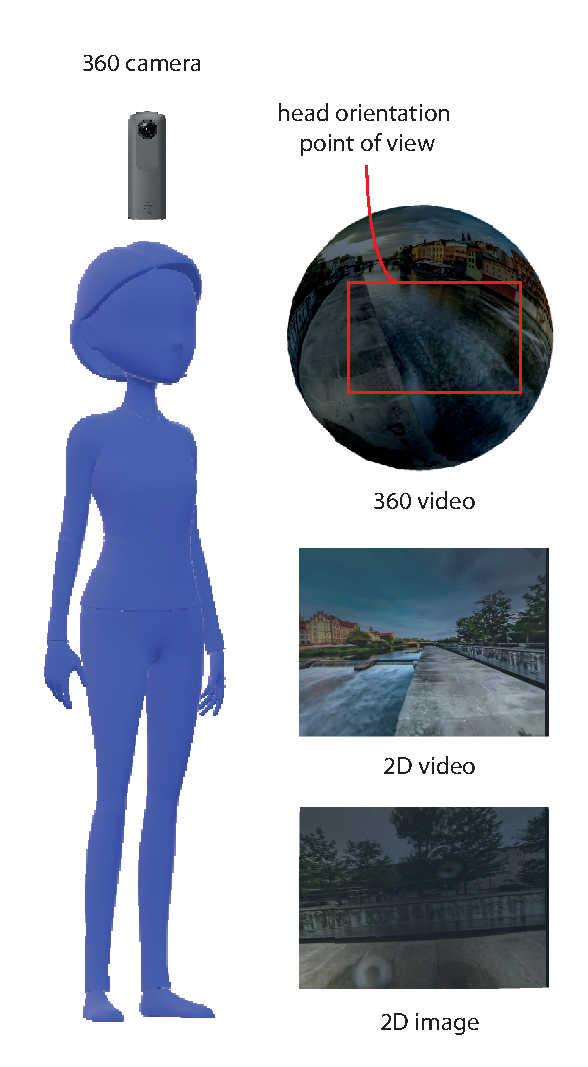
\includegraphics[width=1.5in]{images/chi/images-04.eps}
    \caption{Sharing point of view with different fidelity of representation.}
    \label{fig:data:sharer}
\end{figure}

An example use-case scenario for filtering by sharer is where the sharer is going on a hike and wanting to share the experience of being in an interesting place such as near a river. The sharer takes a live 360-degree video of the surrounding environment and shares it with her followers. The sharer then gets to see how the followers are able to see the shared data based on their social relationship to her. The sharer's intimate friends and family will see the live 360-degree video, other friends the 2D video, and strangers still images of the scene, all automatically created from the 360-degree video recording.

% =============================================================================
\subsection{Viewing Shared Social Data}
% =============================================================================

The user viewing the shared data (the viewer) uses a wearable AR interface to see content from their social network superimposed over the real world, based on proxemics. For example, the viewer may be interested in seeing what their social contacts (followers) are up to and the places they have been. In this scenario the viewer can look around through the AR display to see their social contacts placed around them in three circles ordered by relationship. On top of each social contact, the viewer can see the content they are sharing, filtered based on the social relationship between the social contact and the viewer.

Based on our earlier work \cite{Nassani2017a}, the people who are socially closer will appear in the AR view visually closer and have a more realistic representation. The content shared by each social contact will appear above their avatar (see Figure \ref{fig:data:viewer}), and to view the content more clearly, the user can select it (e.g., using the HoloLens air-tap gesture) to bring the content closer or walk to move inside the 360-degree video sphere. The user can then tap again to bring back the content to its original place to see other social contacts. 

\begin{figure}[ht]
    \centering
    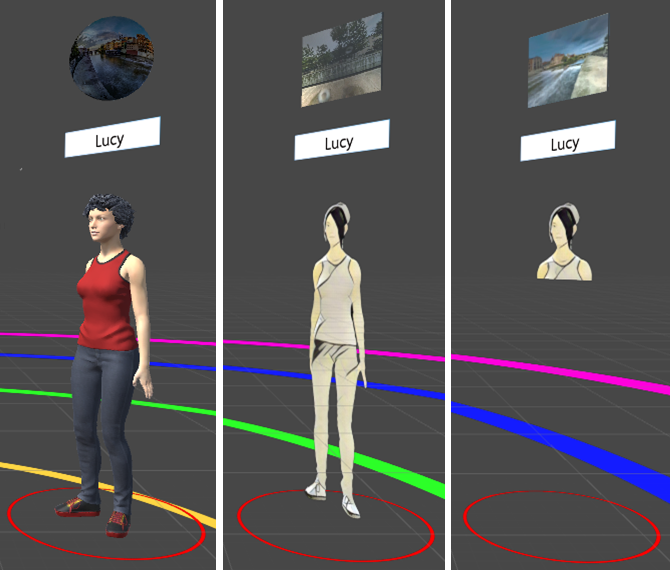
\includegraphics[width=3in]{images/chi/3_levels_of_data.png}
    \caption{Social contact sharing in different relationships with the viewer (Left to right: Intimate, Friend, Stranger). The shared data content (above the avatar) is filtered (360-degree video, 2D video, 2D image) based on social relationship.}
      \label{fig:data:viewer}
\end{figure}

In addition to this operation, this section proposes that the viewers can also see the shared content in different fidelity (360-degree videos, 2D videos or images) based on the social relationship with the sharer (Intimate, Friend or Stranger). While the sharer could restrict the fidelity of the shared content based on the social relationship as mentioned earlier, the viewer could also filter the content based on their preference. In order to avoid getting mentally overloaded by seeing too much content in high fidelity, the viewer should be able to choose the preferred fidelity for the shared content from each social contact. This could be achieved either explicitly by choosing a fidelity for each social contact, or implicitly by moving closer to or further from the avatar representing the contact.      

% =============================================================================
\subsection{Prototype}
% =============================================================================

To explore using the Social AR Continuum metaphor for sharing data between social contacts, a prototype was built using the Microsoft HoloLens. The prototype software was built using Unity 3D game engine, and it allows users to view their social contacts on a wearable AR interface. Figure \ref{fig:data:system} shows the structure of the prototype system. 

\begin{figure}[ht]
    \centering
    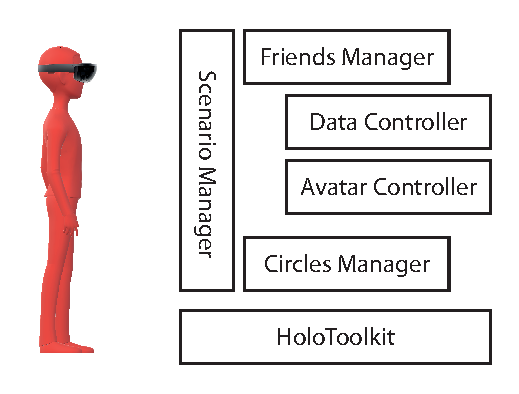
\includegraphics[width=3in]{images/chi/images-03.eps}
    \caption{System components.}
    \label{fig:data:system}
\end{figure}

The prototype places social contacts around the user (viewer) in three concentric circles which are controlled by the \textit{Circles Manager}. The social contacts have different visual fidelity and proximity based on their initial relationship to the viewer, and are rendered using the \textit{Avatar Controller}. The avatars were randomly pre-generated without any resemblance to actual contacts. MakeHuman\footnote{http://www.makehuman.org/} was used to generate the 3D avatars. The viewer (HoloLens user) can turn their head to face different social contacts and then use gestures (air taps) to interact with the contact (view their data or change their position which represents the social relationship). The interactions with HoloLens are enabled using the open-source library \textit{HoloToolkit}\footnote{https://github.com/Microsoft/MixedRealityToolkit-Unity}. The data content shared by the social contacts are controlled by the \textit{Data Controller} which determines which fidelity needs to be displayed based on the social relationship between the avatar and the viewer. The top-level \textit{Scenario Manager} defines the implementation needed for different conditions in the user study, including interaction with avatars, shared data and the concentric circles. 

% =============================================================================
\subsection{User Study}
% =============================================================================

A user study was conducted to test the system usability and effects on social presence, comparing the following conditions: 

\begin{itemize}
    \item C1) Baseline: Shows the shared 360-degree videos from all social contacts.
    \item C2) Tap-to-change: Filters the fidelity of the shared 360-degree videos based on the relationship between the viewer and the social contact. The user can tap on any social contact to cycle through different relationships.
    \item C3) Walk-to-change: Filter the fidelity of the shared 360-degree videos based on the physical distance between the viewer and the social contact.
\end{itemize}

The task was for participants to wear the headset and observe 12 social contacts (mocked up, not reflecting the participant's real social contacts) placed around the user at equal angles from each other to complete a circle (360 degrees) around the viewer, and at different distances to the viewer (centre) based on the social relationship. Each social contact had shared content floating above their head, filtered depending on the type of social relationship that the social contact had with the viewer. 

The participant could view the data content by performing the air-tap gesture on it. Once tapped, the content moved closer to the viewer. For instance, if the viewer tapped on the sphere of a 360-degree video, then the sphere immersed the participant to experience it, while for a 2D video, it was moved closer to the user so they could see it at full-screen resolution.

Participants were asked to answer the 5-point Likert-scale questions shown in Table \ref{tbl:questions} which are based on prior work \cite{Biocca2003}. Participants were asked to rate their experience on the Subjective Mental Effort Questionnaire (SMEQ) \cite{Sauro2009}. 

\begin{figure}[ht]
    \centering
    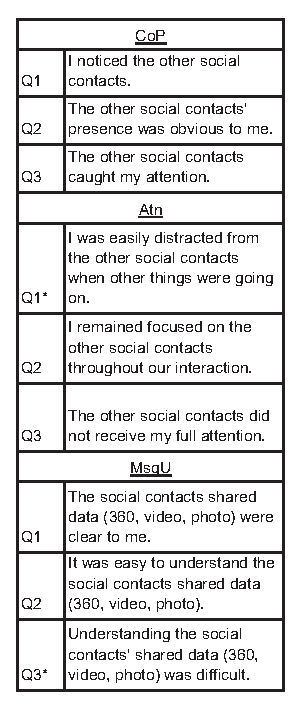
\includegraphics[width=1.5in]{images/chi/images-02.eps}
    \caption{Questionnaires for Social Presence including the following dimensions: CoPresence (CoP), Attentional Allocation (Atn), Perceived Message Understanding (MsgU). *=negative} 
      \label{tbl:questions}
\end{figure}

% =============================================================================
\subsection{Results}
% =============================================================================

A user study was run with eight participants (four female) aged 26-35 (SD=3.03). All participants used social networking platforms on a regular basis, and most (How many?) were familiar with AR/VR displays. 

After filling in a demographic questionnaire, the participants were asked to experience the three conditions in random order. Then they filled in a social presence questionnaire and SMEQ about the condition they just tried. After finishing all three conditions, participants then filled in a post-experiment questionnaire where they were asked about the overall experience and if they had any suggestions to improve it. 

From the questionnaire results (Figure \ref{fig:data:results}), indicates that C2 was rated (3.6) better in terms of social presence compared to C1 (3.3) on average, while C3 (3.5) was relatively close compared to C2. The SMEQ results show that all three conditions were rated low in terms of mental effort, while both C2 (M=16.875) and C3 (M=16.875) were rated lower than C1 (M=21).

\begin{figure}[h]
  \centering
  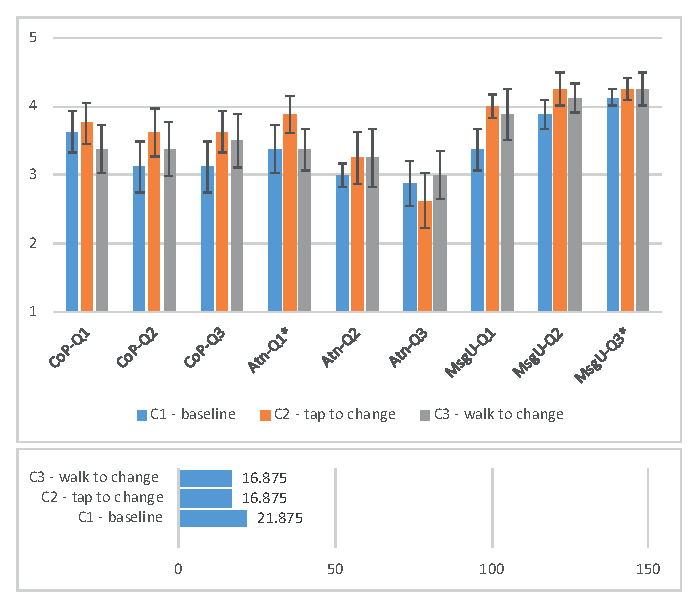
\includegraphics[width=\columnwidth]{images/chi/images-01.eps}
  \caption{Results of social presence (top) and SMEQ (bottom). *=reversed rating scale. Whiskers=standard error}
  \label{fig:data:results}
\end{figure}

As part of the post-questionnaire, participants were asked to rate the three conditions (1=least preferred, 3=most preferred). The ranking results (see Figure \ref{fig:data:ranking}) show that C1 was least preferred (1.3) while C2 (2.25) and C3 (2.375) were similar. There was a statistically significant difference in ranking conditions $\chi^2(2)=7, p=0.05$. A post-hoc analysis with Wilcoxon signed-rank tests was conducted, finding a statistically significant difference between C1-baseline and C3-Walk to change. ($Z=-2.081, p=0.037$), and no difference between the other conditions.

\begin{figure}[h]
  \centering
  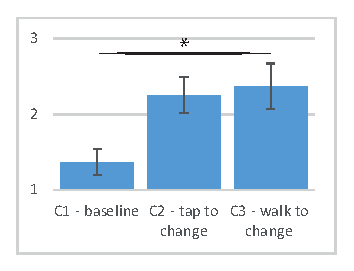
\includegraphics[width=1.5in]{images/chi/images-05.eps}
  \caption{Condition ranking results. Reverse rating scale: 1=least preferred, 3=most preferred. Whiskers=standard error. $*=$ statistically significant difference (Friedman test: $X^2(2)=7, p<0.05$).}  
      \label{fig:data:ranking}
\end{figure}

% =============================================================================
\subsection{Discussion}
% =============================================================================

From a semi-structured interview after the experiment, most users found that condition C3 (walk to change) was a more fun and natural way to view shared data from social contacts. "I feel it is more real and fun to view the 360 videos by walking toward the avatar". Also, other subjects found that the walking condition was more suitable for an outdoor or open area to avoid running into obstacles while walking. The condition C2 (tap to change) was found more convenient for changing the relationship rather than requiring more physical effort, such as walking. The Baseline condition (C1) was the least favourite for participants, as it was too overwhelming having all 360-degree videos shown all around. 

On the downside, participants mentioned some weakness for condition C2 (tap to change), such as potential clutter by being able to bring all social contacts into a small area of the intimate circle. While condition C3 (walk to change) did not have that issue, it was mentioned that by walking one might accidentally change the relationship with other social contacts that the user was not focusing on. For example, the avatars behind or on either side of the user would be affected by user movement, even if the user did not intend to get close to them. Viewing 360-degree videos through an optical see-through display was considered not as ideal, as the 360-degree videos appear to be semi-transparent on top of the real environment.

Overall, participants expressed their interest in using such a system to manage and view their social contacts and shared content in AR, and that it would be useful and easy to use. 

% =============================================================================
\subsection{Limitations and Future Work}
% =============================================================================

This prototype used asynchronous sharing, where social contacts were not online at the same time, sharing live data; the shared content was previously prepared, and the 360-degree videos were previously processed to extract 2D video and a 2D image. However, the method was applied for filtering could be applied to synchronous sharing as well. In the future, the plan is to add live video streaming from social contacts and live scaling down of the content based on social relationships. 

% The concept does apply to synchronous sharing where social contacts are online at the same time. Future plans includes extending this prototype for synchronous sharing experiences. We can expand the implementation to include spatial audio as a fidelity option on which to filter based on social relationship. 

% Additionally, we will conduct a full quantitative and qualitative user study to measure the effects of filtering content type on social presence and user experience. 

% =============================================================================
\subsection{Conclusions}
% =============================================================================

This section presented a mechanism for presenting shared data content by filtering the content type based on the social relationships between the user and the social contacts. 

This work includ an implementation on HoloLens prototype for applying the proposed method in an asynchronous collaboration scenario and conducted a user study using the prototype. The study compared three conditions: viewing 360-degree video without filtering, filtering based on the social relationship, and filtering based on distance.

Initial results showed a trend of participants favouring having the option to filter data over not filtering. The results included a qualitative feedback that provides insights for future directions. 
